\documentclass{beamer}

\usetheme{Copenhagen}
\usepackage[utf8]{inputenc}
\usepackage{graphics}

% Slayt basliklarinda kullanilan font boyutu
\setbeamerfont{frametitle}{size=\normalsize}

\title{Nokta İşlemleri}
\author{Nurettin Şenyer}
\date{Şubat, 2011}
\institute[2011]{19/x}

\begin{document}

\frame{\titlepage}

\frame {
	\frametitle{İçindekiler}
	\begin{itemize}
		\item Resim Temsili
		\item Cebre Ait Temel Kavramlar
		\item Geometrik Dönüşümler
	\end{itemize}
}

\frame {
	\frametitle{Resim Temsili}

	\begin{columns}
		\column{0.6\textwidth}
		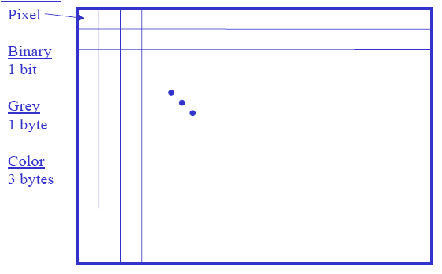
\includegraphics[width=0.9\textwidth]{img/01-repr.png}

		\column{0.4\textwidth}
		\begin{itemize}
			\item Resim == Matris; Piksel == Eleman == Calc:hücre
			\item :: Matrisler vektörlerden oluşur-Cebir
			\item Her bir piksel parlaklık değeriyle ölçülür
			\item :: sensör üzerine düşen ışık miktarı
			\item :: demo: $ccd\_anim.gif$
		\end{itemize}
	\end{columns}
}

\frame {
	\frametitle{Resim Temsili}

	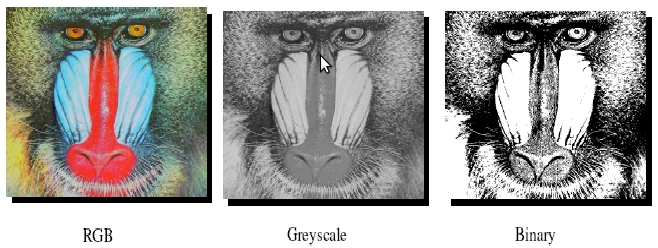
\includegraphics[width=0.9\textwidth]{img/02-rgb-gray-bw.png}
}

\frame {
	\frametitle{Vektörler}

	Sayılar kümesi: $x \in R^n$, $x = [x_1, x_2, ..., x_n]^T$

	\begin{columns}
		\column{0.5\textwidth}
			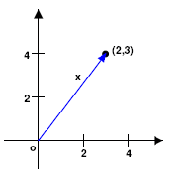
\includegraphics[width=0.9\textwidth]{img/03-vec.png}
		\column{0.5\textwidth}
			Örnek: noktanın koordinat gösterimi
	\end{columns}
}

\frame {
	\frametitle {Vektörler}

	\begin{columns}
		\column{0.5\textwidth}

			\begin{itemize}
				\item 2D Vektör: $\mathbf{v} = (x_1, x_2)$
				\item Genlik: $||v|| = \sqrt{x_1^2 + x_2^2}$
				\item Eğer $||v||=1$ ise, \textbf{BİRİM} vektör
				\item Açı değeri $\theta = \tan^{-1}\left (\frac{x_2}{x_1}\right )$
			\end{itemize}

		\column{0.5\textwidth}
			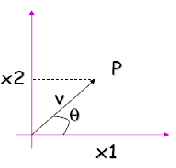
\includegraphics[width=0.9\textwidth]{img/03-vec2.png}
	\end{columns}
}

\frame {
	\frametitle {Vektörler: Toplama}

	\begin{columns}
		\column{0.5\textwidth}
			$v + w = (x_1,x_2) + (y_1,y_2) = (x_1 + y_1, x_2 + y_2)$
		\column{0.5\textwidth}
			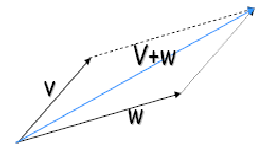
\includegraphics[width=0.9\textwidth]{img/04-vec-add.png}
	\end{columns}
}

\frame {
	\frametitle {Vektörler: Çıkartma}

	\begin{columns}
		\column{0.5\textwidth}
			$v - w = (x_1,x_2) - (y_1,y_2) = (x_1 - y_1, x_2 - y_2)$
		\column{0.5\textwidth}
			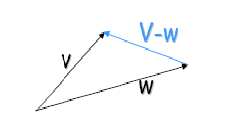
\includegraphics[width=0.9\textwidth]{img/04-vec-sub.png}
	\end{columns}
}

\frame {
	\frametitle {Vektörler: Çarpma}

	\begin{columns}
		\column{0.5\textwidth}
			$a \cdot v = a \cdot (x_1,x_2) = (a \cdot x_1, b \cdot x_2)$
		\column{0.5\textwidth}
			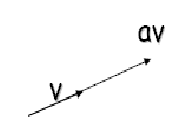
\includegraphics[width=0.9\textwidth]{img/04-vec-prod.png}
	\end{columns}
}

\frame {
	\frametitle {Vektörler: İç (nokta) çarpımı}

	\begin{columns}
		\column{0.5\textwidth}
			$v \cdot w = (x_1,x_2) \cdot (y_1,y_2) = x_1 \cdot y_1 + x_2 \cdot
			y_2$
			\medskip

			İç çarpım sonucu \textbf{SKALAR}
			\medskip

			$v \cdot w = (x_1,x_2) \cdot (y_1,y_2) = ||v|| \cdot ||w|| \cdot
			cos\alpha$
			\medskip

			$v \cdot w = 0 \Leftrightarrow v \perp w$
		\column{0.5\textwidth}
			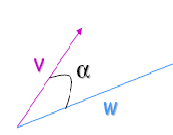
\includegraphics[width=0.9\textwidth]{img/06-vec-inner.png}
	\end{columns}

	\begin{example}
		v=[1 2 3]; w=[4 5 6]; dot(v,w), v * w'
	\end{example}
}

\frame {
	\frametitle {Vektörler}

	Bir noktanın diğerine yansıtılması (iz düşürülmesi),

	\begin{columns}
		\column{0.5\textwidth}
			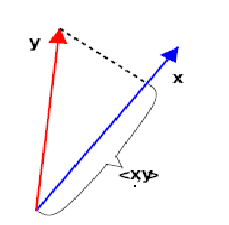
\includegraphics[width=0.9\textwidth]{img/07-vec-proj.png}
		\column{0.5\textwidth}
			farklı gösterimler vardır: $<x,y>$, $x^T y$, $x y$ veya $x \cdot y$
	\end{columns}
}

\frame {
	\frametitle {Doğrusal Bağımlılık}

	\begin{columns}
		\column{0.5\textwidth}
			Eğer $x_3$, $x_1$ ve $x_2$'nin doğrusal kombinasyonuyla elde
			edilebiliyorsa \textbf{doğrusal bağımlıdır} denilir.

		\column{0.5\textwidth}
			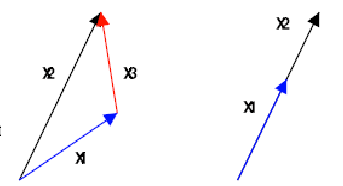
\includegraphics[width=0.9\textwidth]{img/07-linear-dep.png}
	\end{columns}
}

\frame {
	\frametitle {Baz}

	\begin{itemize}
		\item tüm uzayı tarayan, doğrusal bağımsız vektörler kümesi \textbf{baz}
		olarak adlanır.

		\item bu uzayda ki her vektör, bu bazların doğrusal kombinasyonuyla
		yazılabilir

		\item $R^n$'de $n$ doğrusal bağımsız vektör kümesi, $R^n$'nin bazıdır

		\item Eğer $dot(x, y)=0$ ise $x$ ve $y$ \textbf{orthogonaldir}

		\item aynı zamanda $||x|| = ||y|| = 1$ ise \textbf{orthonormaldir}

		\item baz vektörleri orthogonaldir ve eğer birim uzunlukluysalar
		orthonormaldir
	\end{itemize}

	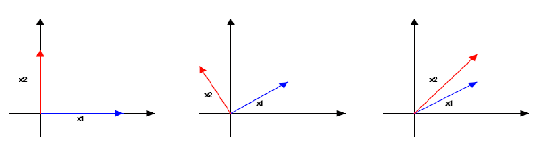
\includegraphics[width=0.9\textwidth]{img/08-basis.png}
}

\frame {
	\frametitle {Baz}

	\begin{itemize}
		\item $R^n$'deki standart bazları (birim vektörler)
		\item :: ${e_i \in R^n : e_i = (0,...,0,1,0,...,0)}$
		\item :: yani $i$. elemanı hariç $0$'dır
		\item herhangi bir vektörü standart bazlar cinsinden şöyle yazarız
		\item :: $[4 7 3]^T = 4 \cdot e_1 + 7 \cdot e_2 + 3 \cdot e_3$
		\item kısaca: $x_i = dot(x, e_i)$ yani vektörü baza yansıt
		\item Benzer kavram: FFT:sinüslere ayrıştırma
		\item Benzer kavram: DCT bazları
	\end{itemize}

	\begin{example}
		x = [4 7 3]; e1 = [1 0 0]; e2 = [0 1 0]; e3 = [0 0 1]; dot(x, e1)
	\end{example}
}

\frame {
	\frametitle {Baz}

	\begin{columns}
		\column{0.5\textwidth}
			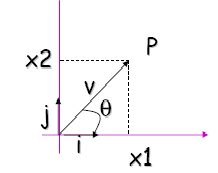
\includegraphics[width=0.9\textwidth]{img/09-orth.png}

		\column{0.5\textwidth}
			$i=(1,0), ||i||=1$
			\medskip

			$j=(0,1), ||j||=1$
			\medskip

			$dot(i, j) = 0$
	\end{columns}

	$v = (x_1, x_2) = x_1 \cdot i + x_2 \cdot j$
	\medskip

	$v \cdot i = ... = x_1$
	\medskip

	$v \cdot j = ... = x_2$
}

\frame {
	\frametitle {Vektörler: çapraz çarpım}

	\begin{columns}
		\column{0.5\textwidth}
			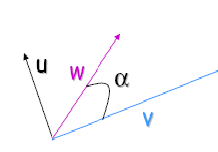
\includegraphics[width=0.9\textwidth]{img/10-cross.png}

		\column{0.5\textwidth}
			$u = v \times w$
			\medskip

			Çapraz çarpım \textbf{VEKTÖR} üretir.
	\end{columns}

	\begin{itemize}
		\item Genlik: $||u|| = ||v \cdot w|| = ||v|| \cdot ||w|| \cdot sin
		\alpha$

		\item Yön: $u \perp v \Rightarrow u \cdot v = (v \times w) \cdot v = 0$
		\item Yön: $u \perp w \Rightarrow u \cdot w = (v \times w) \cdot w = 0$

		\item Yani $u$, hem $v$ hem de $w$'ye diktir.
	\end{itemize}

	\begin{alertblock}{Dikkat}
		$x \times y$ ile $y \times x$ birbirinden farklıdır!
	\end{alertblock}

	\begin{example}
		v = [1 2 3]; w = [4 5 6]; u = cross(v, w)
	\end{example}
}

\frame {
	\frametitle {Matrisler: Toplama}

	Toplama: $C_{nxm} = A_{nxm} + B_{nxm}$

	\begin{example}
		[2 5; 3 1] + [6 2; 1 5]
	\end{example}
}

\frame {
	\frametitle {Matrisler: Çarpma}

	Çarpma: $C_{nxp} = A_{nxm} + B_{mxp}$
	\medskip

	Görüntülerde genelde nokta çarpımı kullanılır ve $A$ resimse, $B$ maskedir

	\begin{example}
		[2 5; 3 1] .* [6 2; 1 5]
	\end{example}

	Ayrıca: transpoze, determinant ($det$), ters hesaplaması ($inv$)
}

\frame {
	\frametitle {Matrisler: rank}

	\begin{itemize}
		\item matrisin rankı, doğrusal bağımsız satır veya sütun sayısıdır

		\item Ör. $rank([1 1; 0 1])$ matrisi $2$ rankına sahipken,
				  $rank([2 1; 4	2])$ matrisi $1$ rankına sahiptir

		\item matris tam ranklıysa, \textbf{non-singular} (tekil olmayan)
		adlanır

		\item tekil matrisin determinantı $0$'dır
	\end{itemize}
}

\frame {
	\frametitle {Özdeğer ve Özvektörler}

	\begin{itemize}
		\item $\lambda \in R$ olmak koşuluyla
		\item :: $A \cdot x = \lambda \cdot x$
		\item eşitliğini sağlayan sıfırdan farklı tüm $x$ vektörlerine $A$'nın
		özvektörü denir

		\item $\lambda$ ise ilişkili özdeğerdir

		\item burada özvektörün, Matrisi bir skalarla
		eşleştirdirdiğine/indirgediğine dikkat edin
		\item :: $MATRIS \cdot x = SKALAR \cdot x \Leftrightarrow MATRIS ==
		SKALAR$
	\end{itemize}
}

\frame {
	\frametitle {Özdeğer ve Özvektörler}

	\begin{itemize}
		\item Eşitliği düzenlersek,
		\item :: $(A - \lambda \cdot I) \cdot x = 0$
		\item buna karakteristik polinom denir

		\item burada $x \neq 0$ olduğundan ve $A - \lambda \cdot I$ tam ranklı
		olması mümkün olmadığından, $det(A - \lambda \cdot I) = 0$ olmalıdır

		\item Eğer $B = T\{A\}$ ise (aralarında doğrusal ilişki varsa)
		karakteristik polinomları \textbf{aynıdır}

		\item bu polinomun kökleri özdeğerleri verir

		\item özdeğerler yerine konulduğunda özvektör elde edilir
	\end{itemize}

	\begin{example}
		A = [2 3; 2 1]; [V, D] = eig(A)
	\end{example}
}

\frame {
	\frametitle {Özdeğer Ayrıştırma}

	\begin{itemize}
		\item Her gerçel, kare, simetrik $A$ matrisi,
		\item :: $A = V \cdot D \cdot V^T$
		\item biçiminde ayrıştırılabilir. Burada $V$ özvektörleri, $D$
		özdeğerleridir
		\medskip

		\item Özdeğer Ayrıştırma, Tekil Değer Ayrıştırmanın (SVD), kısıtlı versiyonudur
	\end{itemize}

	\begin{example}
		A = [2 3; 2 1]; [V, D] = eig(A); V * D * V'
	\end{example}
}

\frame {
	\frametitle {Tekil Değer ($\approx$ özdeğer) Ayrıştırma (SVD)}

	\begin{itemize}
		\item $A \in R^{nxm}$ iken,
		\item :: $A \cdot v = \lambda \cdot u$ ve $A^T \cdot u = \lambda \cdot v$
		\item şartını sağlayan (burada $u \in R^n$ ve $v \in R^m$) $u$ ve $v$
		varsa,
		\item $\lambda \leq 0$'a $A$'nın \textbf{tekil değeri} denilir
		\medskip

		\item Herhangi bir $A \in R^{nxm}$ matrisi
		\item :: $A = U \cdot \sum \cdot V^T$
		\item biçiminde ayrıştırılabilir burada $U \in R^{mxm}$ ve $V \in
		R^{nxn}$ ve orthonormaldir.
		\item $\sum$ ise tekil değerler matrisidir
	\end{itemize}
}

\frame {
	\frametitle {Tekil Değer Ayrıştırma (SVD)}

	\begin{itemize}
		\item :: $A = U \cdot \sum \cdot V^T$
		\item $L = AA^T$ ve $C = A^TA$ dersek
		\item $V$ matrisi $L$'nin ve $U$ matrisi $C$'nin özvektörleridir ve
		\item $u_i = A \cdot v_i$ ilişkisi vardır
	\end{itemize}
	\medskip

	$A = U \cdot \sum \cdot V^T$ ifadesindeki $U, \sum ve V$'nin Hesap Aşamaları:

	\begin{itemize}
		\item $L=AA^T$ ve $C=A^TA$ matrislerini hesapla
		\item $[V, D] = eig(L veya C)$ özdeğer/özvektörleri hesapla
		\item $L$'nin özvektörü $U$, $C$'nin özvektörü $V$'dir
		\item $\sum$'ı elde etmek için, özdeğerleri büyükten küçüğe doğru
			sırala (mutlak genlik olarak), karekökünü hesapla, köşegene yerleştir
		\medskip

		\item "reduced SVD" nedir? Çalışma sorusu
	\end{itemize}
}

\frame {
	\frametitle {Geometrik Dönüşümler: 2D Kayma}

	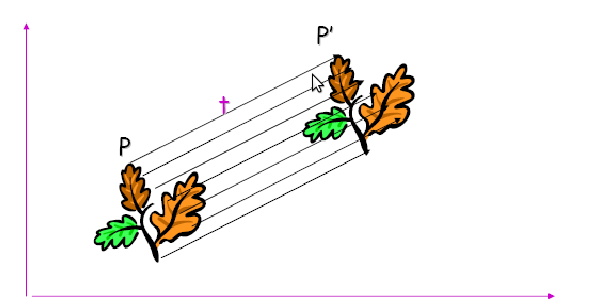
\includegraphics[width=0.9\textwidth]{img/11-trans.png}

	Bu işin iki yönü var: görüntüyü kaydırma, görüntüdeki kaymayı belirle
}

\frame {
	\frametitle {Geometrik Dönüşümler: 2D Kayma: eşitlik}

	\begin{columns}
		\column{0.5\textwidth}
			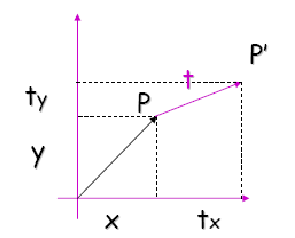
\includegraphics[width=0.9\textwidth]{img/11-trans-eq.png}
		\column{0.5\textwidth}
			$P = (x, y)$ ve $t = (t_x, t_y)$
	\end{columns}
	\medskip

	$P' = (x + t_x, y + t_y) = P + t$
}

\frame {
	\frametitle {Geometrik Dönüşümler: 2D Kayma: matris}

	\begin{columns}
		\column{0.5\textwidth}
			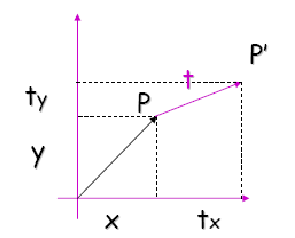
\includegraphics[width=0.9\textwidth]{img/11-trans-eq.png}
		\column{0.5\textwidth}
			$P = (x, y)$ ve $t = (t_x, t_y)$
	\end{columns}
	\medskip

	$P' \rightarrow \begin{bmatrix}
		x + t_x\\
		y + t_y \end{bmatrix} = \begin{bmatrix}
			1 & 0 & t_x\\
			0 & 1 & t_y
		\end{bmatrix} \cdot \begin{bmatrix}
			x\\y\\1
		\end{bmatrix}$
}

\frame {
	\frametitle {Geometrik Dönüşümler: homojen koordinatlar}

	kartezyen - homojen koordinat dönüşümü
	\medskip

	$(x, y)    \rightarrow (x \cdot z, y \cdot z, z), z \neq 0$
	$(x, y, z) \rightarrow (x \cdot w, y \cdot, z \cdot w, w), w \neq 0$
	\medskip

	$(t_x, t_y) \rightarrow (t_x, t_y, 1)$
	\medskip

	Ters dönüşüm
	\medskip

	$(x,y,z), z \neq 0 \rightarrow (x/z, y/z)$
	$(x,y,z,w), w \neq 0 \rightarrow (x/w, y/w, z/w)$
}

\frame {
	\frametitle {Geometrik Dönüşümler: kayma: homojen}

	\begin{columns}
		\column{0.5\textwidth}
			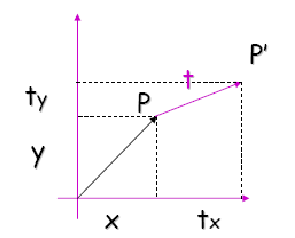
\includegraphics[width=0.9\textwidth]{img/11-trans-eq.png}
		\column{0.5\textwidth}
			$P = (x, y) \rightarrow (x,y,1)$ ve $t = (t_x, t_y) \rightarrow (t_x
			t_y, 1)$
	\end{columns}
	\medskip

	$P' \rightarrow \begin{bmatrix}
		x + t_x\\
		y + t_y\\
		1\end{bmatrix} = \begin{bmatrix}
			1 & 0 & t_x\\
			0 & 1 & t_y\\
			0 & 0 & 1
		\end{bmatrix} \cdot \begin{bmatrix}
			x\\y\\1
		\end{bmatrix}$
	\medskip
	$P' = T \cdot P$
}

\frame {
	\frametitle {Geometrik Dönüşümler: ölçekleme}

	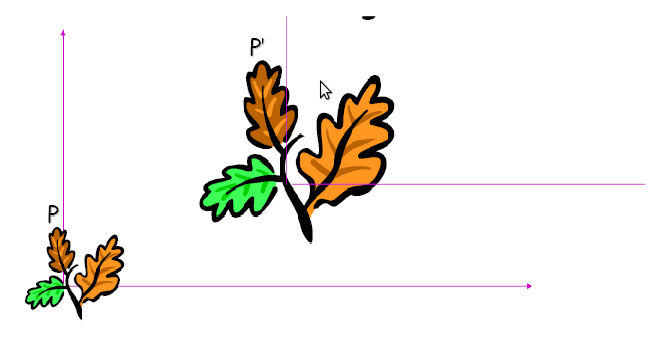
\includegraphics[width=0.9\textwidth]{img/14-scale.png}
}

\frame {
	\frametitle {Geometrik Dönüşümler: ölçekleme: eşitlik}

	\begin{columns}
		\column{0.5\textwidth}
			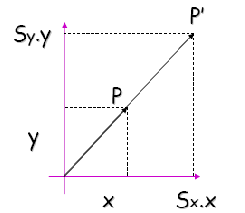
\includegraphics[width=0.9\textwidth]{img/14-scale-eq.png}
		\column{0.5\textwidth}
			$P = (x, y) \rightarrow (x,y,1)$ ve $P' = (s_x \cdot x, c_y \cdot y,
			y) \rightarrow (s_x \cdot x, s_y \cdot y, 1)$
	\end{columns}
	\medskip

	$P' \rightarrow \begin{bmatrix}
		s_x \cdot x\\
		s_y \cdot y\\
		1\end{bmatrix} = \begin{bmatrix}
			s_x & 0 & 0\\
			0 & s_y & 0\\
			0 & 0 & 1
		\end{bmatrix} \cdot \begin{bmatrix}
			x\\y\\1
		\end{bmatrix}$
	\medskip
	$P' = S \cdot P$
}

\frame {
	\frametitle {Geometrik Dönüşümler: ölçekle - kaydır}

	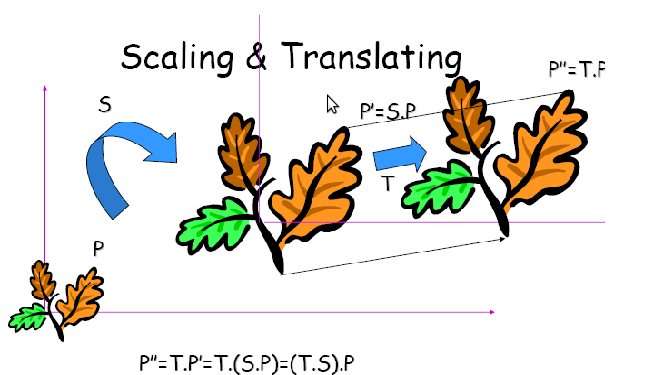
\includegraphics[width=0.9\textwidth]{img/15-scale-trans.png}

	\medskip
	$P'' = T \cdot P' = T \cdot (S \cdot P) = (T \cdot S) \cdot P$
}

\frame {
	\frametitle {Geometrik Dönüşümler: ölçekle - kaydır: eşitlik}

	$P'' = T \cdot P' = T \cdot (S \cdot P) = (T \cdot S) \cdot P$
	\medskip

	$P'' = T \cdot S \cdot P = \begin{bmatrix}
		1 & 0 & t_x\\
		0 & 1 & t_y\\
		0 & 0 & 1
	\end{bmatrix} \cdot \begin{bmatrix}
		s_x & 0   & 0\\
		0   & s_y & 0\\
		0   & 0   & 1
	\end{bmatrix} \cdot \begin{bmatrix}
		x\\y\\1
	\end{bmatrix}$
	\medskip

	$P'' = \begin{bmatrix}
		s_x & 0   & t_x\\
		0   & t_y & t_y\\
		0   & 0   & 1
	\end{bmatrix} \cdot \begin{bmatrix}
		x\\y\\1
	\end{bmatrix} = \begin{bmatrix}
		s_x \cdot x + t_x\\
		s_y \cdot y + t_y\\
		1
	\end{bmatrix}$
}

\frame {
	\frametitle {Geometrik Dönüşümler: sıra önemlidir}

	$P'' = S \cdot T \cdot P \neq T \cdot S \cdot P$
}

\frame {
	\frametitle {Geometrik Dönüşümler: dönme}

	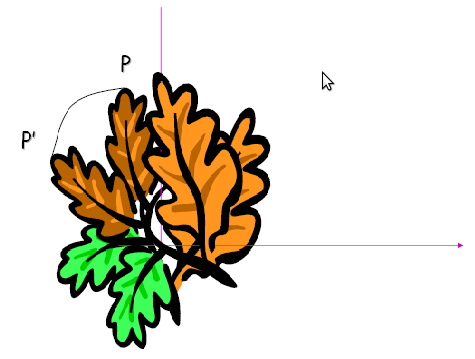
\includegraphics[width=0.9\textwidth]{img/16-rot.png}
}

\frame {
	\frametitle {Geometrik Dönüşümler: dönme: eşitlik}

	$\theta$ açısı kadar saat yönünde döndür,

	\begin{columns}
		\column{0.5\textwidth}
			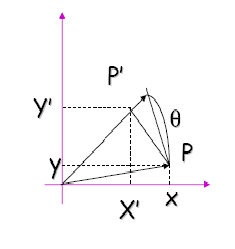
\includegraphics[width=0.9\textwidth]{img/16-rot-eq.png}

		\column{0.5\textwidth}
			$\begin{bmatrix}
			x'\\y'\end{bmatrix} = \begin{bmatrix}
			cos \theta & -sin \theta\\
			sin \theta & cos \theta
			\end{bmatrix} \cdot \begin{bmatrix}
			x\\y
			\end{bmatrix}$
	\end{columns}
	\medskip
	$P' = R \cdot P$
}

\frame {
	\frametitle {Geometrik Dönüşümler: 3D dönme}

	Koordinat ekseni etrafında, saat yönünde döndür

	\begin{columns}
		\column{0.5\textwidth}
			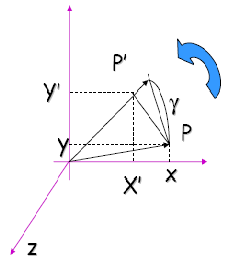
\includegraphics[width=0.9\textwidth]{img/17-3d-rot.png}
		\column{0.5\textwidth}
			$R_x(\alpha) = \begin{bmatrix}
				1 & 0 & 0\\
				0 & cos \alpha & -sin \alpha\\
				0 & sin \alpha & cos \alpha
			\end{bmatrix}$
			...
	\end{columns}
}

\end{document}
